\documentclass{beamer}

\usepackage{amsmath}
\usepackage{xcolor}
\usepackage{graphicx}
\usepackage{cite}
\usepackage{subcaption}
\usepackage{amsmath}
\usepackage{pgfplots}
\usepackage[absolute,overlay]{textpos}



\usepackage{ragged2e}
\justifying

\usetheme[progressbar=frametitle]{metropolis}
\setbeamertemplate{frame numbering}[fraction]
\useoutertheme{metropolis}
\useinnertheme{metropolis}
\usefonttheme{metropolis}
\usecolortheme{spruce}
\setbeamercolor{background canvas}{bg=white}

%\usetheme{Warsaw}
%\usecolortheme{crane}
\definecolor{mygray}{rgb}{0.3,0.3,0.3}
\usecolortheme[named=mygray]{structure}


\title[Reinforcement Learning]{A Self-organized Sensor Data Path Selection Method in Internet of Things}
\author{Researcher: Milad Khademi Nori \\ Supervisors: Saeed Sharifian \& Amirhossein Rezaei}
\institute{Electrical Engineering Department at Amirkabir University of Technology}
\date{\today}
\begin{document}

\begin{frame}
\titlepage
\end{frame}


\begin{frame}[t]{Agenda} %\vspace{10pt}

\begin{itemize}
\item Internet of Things (IoT)
		\begin{itemize}
		\item Why IoT? \& What is IoT?
		\item Layers of IoT \& Our Intended (Studied) Layer
		\item Sensor Data Path Selection Problem
		\end{itemize}		
\item Current Protocols for Sensor Data Path Selection Problem
		\begin{itemize}		
		\item Non-classic Protocols \& Their Pros and Cons
		\item Classics Protocols \& Their Pros and Cons
	%	\item Can a Protocol Have Both?
		\item Literature Review
		\end{itemize}		
\item Our Proposed Protocol
		\begin{itemize}
		\item Euclidean Distance Matrix (EDM) \& Low-rank Matrix Reconstruction with Noise
		\end{itemize}
\item Simulations
\item Conclusion
\end{itemize}
\end{frame}


\begin{frame}[t]{Internet of Things} %\vspace{10pt}

\begin{textblock}{0.5}(6.3,5.5)
\includegraphics[scale=0.2]{figure/kevin1.png}
\end{textblock}


\begin{itemize}

\item Why IoT?

\begin{itemize}
\justifying
\item Information is a great way to reduce waste and increase efficiency, and that's really what the internet of things provides.
\end{itemize}

\item What is IoT?

\begin{itemize}
\justifying
\item The (IoT) is the \hspace{70pt} extension of internet   connectivity into \hspace{100pt} physical devices and everyday objects.
\end{itemize}

\item Layers of IoT

\begin{itemize}
\justifying
\item Things (Sensors)
\item Connectivity
\item Applications
\end{itemize}

\end{itemize}
\end{frame}


\begin{frame}[t]{Things (Sensors) Layer} %\vspace{10pt}

\begin{textblock}{0.5}(7.2,2)
\includegraphics[scale=0.5]{figure/Things.png}
\end{textblock}

\begin{itemize}
\justifying
\footnotesize
\item Things are our worlds \\ digital nervous system, hence, \\ the major task of things \\ is to gather all of the \\ environmental parameters, \\ aggregate and forward \\ them to the Base Station \\ (BS) which is the gateway \\ to the connectivity layer or internet backbone using a variety of routing protocols [1].

\item Obstacles

\begin{itemize}

\footnotesize

\item Occasional energy shortage

\item Stochastic nature of Energy Harvesting Rate.

\item A need for an efficient protocol [2]

\begin{textblock}{0.5}(11,9.5)
\includegraphics[scale=0.2]{figure/NodeFig.PNG}
\end{textblock}

\end{itemize}

\end{itemize}
\end{frame}


\begin{frame}[t]{Sensor Data Path Selection Protocol Types} %\vspace{10pt}

\begin{textblock}{0.5}(7.2,2)
\includegraphics[scale=0.5]{figure/Things.png}
\end{textblock}

\begin{textblock}{0.5}(8.4,8.5)
\includegraphics[scale=0.2]{figure/Hierarchical.png}
\end{textblock}


\begin{itemize}
\justifying
\footnotesize

\item Flat protocols

\begin{itemize}
\justifying
\footnotesize
\item In the flat protocols, \\ network works as a \\ whole and all things \\ play the same role [2].
\end{itemize}


\item Hierarchical protocols
\begin{itemize}
\justifying
\footnotesize
\item In the hierarchical \\ protocols, things are \\ partitioned into a number \\ of clusters and some things \\ are used as Cluster Heads \\ abbreviated as CHs [2].

\item Hierarchical protocols \\ outperform flat protocols \\ in term of energy efficiency [2].

\end{itemize}
\end{itemize}
\end{frame}


\begin{frame}[t]{Hierarchical Protocols} %\vspace{10pt} 
\small
\begin{itemize}
\justifying
\item In hierarchical protocols, two decisions mainly determine the energy-efficiency of the protocols [1].
	
\begin{itemize}
\item Clustering
\item Cluster Head Selection
\end{itemize}
	
\item In hierarchical protocols, networks work in consecutive rounds. Each round consists of: 
\begin{itemize}
\item Setup phase
\item Steady-state phase
\end{itemize}

\end{itemize}

\begin{center}
\includegraphics[scale=0.69]{figure/Phase}
\end{center}

\end{frame}


\begin{frame}[t]{Non-classic Protocols \& Classic Protocols} %\vspace{10pt}

\begin{textblock}{0.5}(8.4,8.5)
\includegraphics[scale=0.2]{figure/Hierarchical.png}
\end{textblock}

\small
$\bullet$ Non-classic Protocols (LEACH [3], DEARER [1], EPSO-CEO [4], and WOA-C [5])\\
\quad $\bullet$ {\color{green} They do not rely on GPS.}	\\
\quad $\bullet$ {\color{red} They form inefficient clusters.} \\
\quad $\bullet$ {\color{red} High energy-consumption.} \\
\quad $\bullet$ {\color{red} High energy-shortage.} \\
$\bullet$ Classic protocols (KCA [6] and Mk-means [7])\\
\quad $\bullet$ {\color{green} They can form clusters efficiently.}	\\
\quad $\bullet$ {\color{red} They rely on GPS module [8].} \\
\quad \quad $\bullet$ {\color{red} GPS increases implementation \\ \quad \quad \quad cost [8].}\\
\quad \quad $\bullet$ {\color{red} GPS increases energy  \\ \quad \quad \quad  consumption [8].}\\
\quad \quad $\bullet$ {\color{red} GPS works poorly in indoor  \\ \quad \quad \quad  applications [8].}\\
\end{frame}

\begin{frame}[t]{Literature Review} %\vspace{10pt}
\begin{table}[H]
\footnotesize
\begin{tabular}{|c|c|c|c|c|c|c|c|}
\hline
Protocols & Inter & NGPS & ResEn & HarEn & Cov & Clas & Dis \\ \hline
LEACH 2000 [9]& $\times$ & $\surd$ & $\times$ & $\times$ & $\times$ & $\times$ & $\surd$ \\ \hline
LEACH 2017 [10]& $\surd$ & $\surd$ & $\times$ & $\times$ & $\times$ & $\times$ & $\times$\\ \hline
LEACH 2016 [11]& $\times$ & $\surd$ & $\surd$ & $\times$ & $\times$ & $\times$ & $\times$\\ \hline
LEACH 2016 [12]& $\times$ & $\surd$ & $\times$ & $\times$ & $\surd$ & $\times$ & $\surd$\\ \hline
DEARER 2016 [13]& $\times$ & $\surd$ & $\times$ & $\surd$ & $\times$ & $\times$ & $\times$\\ \hline
GEEC 2015 [14]& $\times$ & $\surd$ & $\surd$ & $\surd$ & $\times$ & $\times$ & $\times$\\ \hline
KASSAN 2018 [15]& $\times$ & $\times$ & $\surd$ & $\times$ & $\times$ & $\times$ & $\times$\\ \hline \hline
K-means 2016 [16]& $\times$ & $\times$ & $\surd$ & $\times$ & $\surd$ & $\surd$ & $\times$\\ \hline
EECPK 2016 [17]& $\times$ & $\times$ & $\surd$ & $\times$ & $\surd$ & $\surd$ & $\times$\\ \hline
Fuzzy 2018 [18]& $\times$ & $\times$ & $\surd$ & $\times$ & $\surd$ & $\surd$ & $\times$\\ \hline
K-medoids 2018 [19]& $\times$ & $\times$ & $\times$ & $\times$ & $\surd$ & $\surd$ & $\times$\\ \hline
EMBEDMENT [20] & {\color{green} $\surd$} & {\color{green} $\surd$} & {\color{green} $\surd$} & {\color{green} $\surd$} &{\color{green} $\surd$} & {\color{green} $\surd$} & {\color{green} $\surd$}\\ \hline
\end{tabular}	
\end{table}
\tiny
Inter: Inter-cluster communication, NGPS: No-GPS, ResEn: Residual energy, HarEn: Harvesting energy, Cov: Coverage, Clas: Classic Clustering, Dis: Distributed
\end{frame}

\begin{frame}[t]{Our Proposed Protocol} %\vspace{10pt}
\begin{center}
\includegraphics[scale=0.5]{figure/Steps.pdf}
\end{center}
\end{frame}

\begin{frame}[t]{First Step} %\vspace{10pt}

\begin{itemize}

\item RSSI measurement

\item RSSI collection

\item Storing RSSI in a \\ vector

\item Send and receive \\ must happen \\ more than 20 times

\end{itemize}

\begin{equation}
        \left\{ \begin{array}{ll}
    		s_{1}=[\cdot]_{(N+1)\times1}     & \textrm{thing number $1$}\\
    	    \vdots                            &\quad \vdots \\
    		s_{i}=[\cdot]_{(N+1)\times1}   & \textrm{thing number $i$}\\
    	    \vdots                            &\quad \vdots \\
    		s_{(N+1)}=[\cdot]_{(N+1)\times1}   & \textrm{thing number $(N+1)$}
        \end{array} \right.
\end{equation}

\begin{textblock}{0.8}(6.3,2.5)
\includegraphics[scale=0.35]{figure/Steps.pdf}
\end{textblock}
\end{frame}


\begin{frame}[t]{Second Step} %\vspace{10pt}

\begin{itemize}

\item RSSI transmission

\item One problem!

\item Low-range

\item An elementary \\ clustering should \\ be performed. \\ This could be \\ LEACH with 10 \% CHs.

\item Flooding

\item BS, in that end, receives all RSSI measurement vectors

\item RSSI helps BS to estimate distances between things
\end{itemize}


\begin{textblock}{0.8}(6.3,2.5)
\includegraphics[scale=0.35]{figure/Steps.pdf}
\end{textblock}
\end{frame}

\begin{frame}[t]{Third Step} %\vspace{10pt}
\small
\begin{itemize}
\item Different Path Loss \\ (PL) models for \\ each environment.

\item Free Space Model

\item Two-Ray Ground \\ Model

\item Log-Normal \\ Shadowing Model

\item These PL models help us to estimate the distance based on the PL which is the difference between TSSI and RSSI [21].
\end{itemize}

\begin{textblock}{0.8}(6.3,2.5)
\includegraphics[scale=0.35]{figure/Steps.pdf}
\end{textblock}
\end{frame}

\begin{frame}[t]{Third Step} %\vspace{10pt}

\footnotesize

$\bullet$ Theoretical Models for PL

\begin{equation}
Free \ Space \ Model: \ PL=20\log (d) +20\log (f) -27.55
\end{equation}


\begin{equation}
Two-Ray \ Ground \ Model: \ PL=40\log (d) -20\log (h_t) -20\log(h_r)
\end{equation}

\begin{equation}
Log-Normal \ Shadowing \ Model: \ PL= PL(d_0)+10n \log(\frac{d}{d_0})+X_{\sigma}
\end{equation}

$\bullet$ Empirical Models for PL

\begin{equation}
Weissberger: \ PL=
        \left\{ \begin{array}{ll} 
    		1.33\times f^{0.284} d^{0.588}     & \quad 14m < d \leq 400m\\
    		0.45\times f^{0.284} d  & \quad 0m \leq d < 14m
        \end{array} \right.
\end{equation}


\begin{equation}
ITU-R: \ PL=0.2 \times f^{0.3}d^{0.6}
\end{equation}

\end{frame}

\begin{frame}[t]{Third Step	} %\vspace{10pt}
\begin{equation}
COST: \ PL=15.6 \times f^{-0.009}d^{0.26}
\end{equation}

\begin{equation}
Proposed: \ PL=X f^{Y}d^{Z}
\end{equation}

\begin{itemize}

\item The empirical method in equation (8) is employed to estimate the distances [21]. More precisely,

\begin{equation}
d=\Big(\frac{PL}{X\times f^Y}\Big)^{1/Z}
\end{equation}

\item Now, we have distances though it maybe inaccurate for long distances which multi-path fading affects them. This inaccuracy could be overcome.

\end{itemize}
\end{frame}

\begin{frame}[t]{Third Step} %\vspace{10pt}

\begin{equation}
        \left\{ \begin{array}{ll}
    		d_{1}=[\cdot]_{(N+1)\times1}     & \textrm{thing number $1$}\\
    	    \vdots                            &\quad \vdots \\
    		d_{i}=[\cdot]_{(N+1)\times1}   & \textrm{thing number $i$}\\
    	    \vdots                            &\quad \vdots \\    		d_{(N+1)}=[\cdot]_{(N+1)\times1}   & \textrm{thing number $(N+1)$}
        \end{array} \right.
\end{equation}

\begin{itemize}

\item Now, the BS knows the distance of each thing to its neighbors

\item The above vectors are sparse because each thing can receive packet from its neighbors.

\item But it needs the distance of each thing to all of the things.
\end{itemize}
\end{frame}

\begin{frame}[t]{Fourth Step} %\vspace{10pt}
\begin{textblock}{0.8}(6.3,2.5)
\includegraphics[scale=0.35]{figure/Steps.pdf}
\end{textblock}

\begin{itemize}

\small

\item Time to obtain \\ the Euclidean \\ distance matrix.

\item A semi-complete \\ matrix.

\item A lot of unknown \\ entries!

\item Unfortunately, known \\ entries are also noisy.

\end{itemize}

\begin{equation}
\hat{D}=[d_{1},d_{2},\cdots,d_{(N+1)}]_{(N+1)\times(N+1)}
\end{equation}

\end{frame}

\begin{frame}[t]{Fifth Step} %\vspace{10pt}

\begin{itemize}

\item GOOD NEWS!

\item "Matrix completion with noise" can reconstruct our matrix [22].

\item It also can denoises our matrix.

\item But how?

\item By solving the following SDP optimization problem:

\begin{equation}
\begin{split}
minimize \quad rank(X) \\
subject \ to \quad ||X-Y||_F \leq \delta
\end{split}
\end{equation}

\item But, this is NP-hard, instead, it is possible to solve the relaxed form of the SDP problem:

\end{itemize}
\end{frame}

\begin{frame}[t]{Fifth Step} %\vspace{10pt}
\begin{equation}
\begin{split}
minimize \quad ||X||_* \\
subject \ to \quad ||X-Y||_F \leq \delta
\end{split}
\end{equation}

\begin{itemize}
\item Which $||X||_*$ the is nuclear norm of $X$, and can be calculated as follows:

\begin{equation}
||X||_*:= \sigma_1+ \sigma_2+ \sigma_3+ \cdots+ \sigma_i+ \cdots+ \sigma_N
\end{equation}

\item We're done. BS can this way reconstruct the semi-complete matrix.

\item But hold on!! It's not that easy.

\end{itemize}
\end{frame}

\begin{frame}[t]{Fifth Step} %\vspace{10pt}
\begin{itemize}
\item Still in the 5th step ...

\item Conditions need to be hold to able to reconstruct accurately and even exactly:

\begin{itemize}
\justifying
\item Exact case: The semi-complete matrix should have $N \times R \times (log \ N)^2$ entries coherently distributed in all of the rows (N: dimension of matrix, R: rank of matrix). Take $N=1000$ and $R=4$ (2D EDM),then having at least 36000 entries is enough to reconstruct other 964000 entries [22]. A miracle!!

\item Accurate case ($ \pm 3 \% $ error reported): Having $N \times R$ entries coherently distributed is enough. Therefore, assuming again $N=1000$ and $R=4$, having at least 4000 entries enough to reconstruct other 996000 entries [22].
\begin{equation}
Complexity \ of \ Reconstruction: \ O(3 \times N \times R^2 + R^3)
\end{equation}
\end{itemize}
\item Now the BS knows the peer-to-peer distances.

\end{itemize}
\end{frame}

\begin{frame}[t]{Sixth Step} %\vspace{10pt}
\begin{textblock}{0.8}(6.3,2.5)
\includegraphics[scale=0.35]{figure/Steps.pdf}
\end{textblock}
\begin{itemize}

\item Clustering takes \\ place.

\item K-medoids handles \\ outliers much \\ more resiliently \\ than k-means.

\item Complexity [23]:

\item $J_{opt}$ clusters [24].

\item They are isolated.

\item Let's connect them.
\begin{equation}
PAM: O(J(N-J)^2)
\end{equation} 
\begin{equation}
J_{opt}=\sqrt{\frac{N \varepsilon_{fs}}{2\pi \varepsilon_{mp}}}\frac{L}{d_{toBS}^{2}}
\end{equation}


\end{itemize}
\end{frame}

\begin{frame}[t]{Seventh Step} %\vspace{10pt}
\begin{textblock}{0.8}(6.3,2.5)
\includegraphics[scale=0.35]{figure/Steps.pdf}
\end{textblock}
\begin{itemize}

\item Minimum spanning \\ tree could connect \\ the clusters [24].

\item Allows far clusters \\ to reach the BS.

\item In the next step, \\ the BS has to \\ select a CH for each \\ cluster.

\item An ILP optimization problem  is formulated to select.

\item Lowest energy-consumption in a round.

\end{itemize}
\end{frame}


\begin{frame}[t]{Eighth Step} %\vspace{10pt}
\begin{equation}
minimize\quad R(\ell)\sum_{i=1}^{C_{j}}x_i(\Lambda_{ij}+\Delta_{ij})
\end{equation}
\begin{equation}
subject\ to\quad \sum_{i=1}^{C_j}x_i\Big(E_i(\ell)+H_i(\ell)-R(\ell)\Delta_{ij}\Big)\geq0
\end{equation}
\begin{equation}
\sum_{i=1}^{C_j}x_i=1, \quad x_i\in \{0,1\}
\end{equation}

\begin{itemize}
\justifying
\item After all of these steps, BS sends a packet to all things, including:
\begin{itemize}
\item Euclidean distance matrix.
\item Cluster membership.
\item The minimum spanning tree.
\item CHs.
\end{itemize}

\end{itemize}


\end{frame}

\begin{frame}[t]{Simulations} %\vspace{10pt}
\begin{itemize}
\small
\justifying
\item Comparison criteria:

\begin{itemize}
\item Energy efficiency [2]
\begin{equation}
\eta=\lim_{L\to\infty}\frac{\sum_{\ell=1}^{L}\sum_{i=1}^{N}P_{i}(\ell)}{\sum_{\ell=1}^{L}\sum_{i=1}^{N}H_{i}(\ell)} \quad (Packet/Joule)
\end{equation}
\item Packet loss [2]
\begin{equation}
\zeta=\lim_{L\to\infty}\frac{\sum_{\ell=1}^{L}\sum_{i=1}^{N}P_{i}(\ell)}{\sum_{\ell=1}^{L}\sum_{i=1}^{N}A_{i}(\ell)} 
\end{equation}

\item Lifetime [3]
\begin{itemize}
\item The passed time until one thing dies.
\end{itemize}
\end{itemize}
\item  Opponents
\begin{itemize}
\item DEARER [2]
	\begin{itemize}
	\item The same assumptions: No GPS
	\end{itemize}
\item K-means [3]
	\begin{itemize}
	\item An additional assumption: Things equipped with GPS
	\end{itemize}
\end{itemize}

\end{itemize}
\end{frame}

\begin{frame}[t]{Scenarios} %\vspace{10pt}

\begin{textblock}{0.8}(0.3,1.75)
\includegraphics[scale=0.371]{figure/Scen1.png}
\end{textblock}

\begin{textblock}{0.8}(8.3,1.75)
\includegraphics[scale=0.371]{figure/Scen2.png}
\end{textblock}

\begin{textblock}{0.8}(4.3,8.8)
\includegraphics[scale=0.371]{figure/Scen3.png}
\end{textblock}

\begin{textblock}{7}(1,9.3)
\small
Uniform distribution
\end{textblock}

\begin{textblock}{3.5}(11.5,9.3)
\small
Gaussian distribution $N(\mu=0,\sigma=100)$
\end{textblock}

\begin{textblock}{3}(1,14)
\small
Gaussian mixture $N(\mu,\sigma=30)$
\end{textblock}

\end{frame}



\begin{frame}[t]{First Scenario} %\vspace{10pt}

\begin{textblock}{3}(1,0.7)
\begin{figure}[!t]
\begin{center}
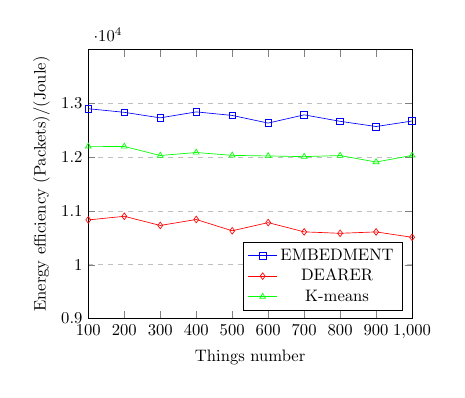
\begin{tikzpicture} [scale = 0.6]
\begin{axis}[
    %title={Energy Efficiency},
    xlabel={Things number},
    ylabel={Energy efficiency (Packets)/(Joule)},
    xmin=100, xmax=1000,
    ymin=9000, ymax=14000,
    xtick={100,200,300,400,500,600,700,800,900,1000},
    ytick={9000,10000,11000,12000,13000},
    legend pos=south east,
    ymajorgrids=true,
    grid style=dashed,
]
 
\addplot[
    color=blue,
    mark=square,
    ]
    coordinates {
    (100,12901)(200,12834)(300,12731)(400,12842)(500,12776)(600,12634)(700,12787)(800,12667)(900,12570)(1000,12672)
    };
    \addlegendentry{EMBEDMENT}
    
\addplot[
    color=red,
    mark=diamond,
    ]
    coordinates {
    (100,10834)(200,10901)(300,10731)(400,10842)(500,10632)(600,10784)(700,10612)(800,10585)(900,10611)(1000,10511)
    };
    \addlegendentry{DEARER}
    
\addplot[
    color=green,
    mark=triangle,
    ]
    coordinates {
    (100,12201)(200,12199)(300,12031)(400,12087)(500,12034)(600,12023)(700,12010)(800,12031)(900,11910)(1000,12033)
    };
    \addlegendentry{K-means}
    
\end{axis}
\end{tikzpicture}
\end{center}
\end{figure}
\end{textblock}

\begin{textblock}{3}(8.2,1.1)
\begin{figure}[!t]
\begin{center}
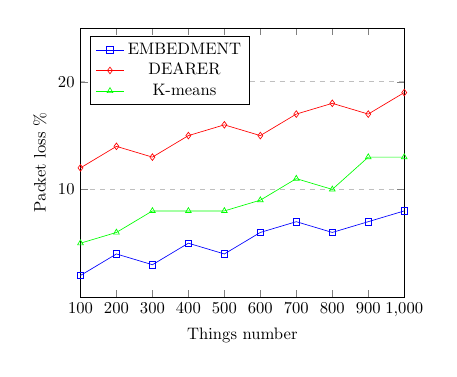
\begin{tikzpicture} [scale = 0.6]
\begin{axis}[
    %title={Packet Fail Percentage},
    xlabel={Things number},
    ylabel={Packet loss \%},
    xmin=100, xmax=1000,
    ymin=0, ymax=25,
    xtick={100,200,300,400,500,600,700,800,900,1000},
    ytick={10,20},
    legend pos=north west,
    ymajorgrids=true,
    grid style=dashed,
]
 
\addplot[
    color=blue,
    mark=square,
    ]
    coordinates {
    (100,2)(200,4)(300,3)(400,5)(500,4)(600,6)(700,7)(800,6)(900,7)(1000,8)
    };
    \addlegendentry{EMBEDMENT}
    
\addplot[
    color=red,
    mark=diamond,
    ]
    coordinates {
    (100,12)(200,14)(300,13)(400,15)(500,16)(600,15)(700,17)(800,18)(900,17)(1000,19)
    };
    \addlegendentry{DEARER}    
    
\addplot[
    color=green,
    mark=triangle,
    ]
    coordinates {
    (100,5)(200,6)(300,8)(400,8)(500,8)(600,9)(700,11)(800,10)(900,13)(1000,13)
    };
    \addlegendentry{K-means}
    
\end{axis}
\end{tikzpicture}
\end{center}
\end{figure}
\end{textblock}


\begin{textblock}{3}(0.7 ,8.1)
\begin{figure}
\begin{center}
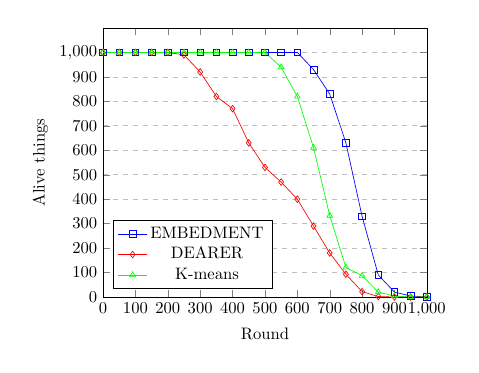
\begin{tikzpicture}[scale = 0.6]
\begin{axis}[
    %title={Packet Fail Percentage},
    xlabel={Round},
    ylabel={Alive things},
    xmin=0, xmax=1000,
    ymin=0, ymax=1100,
    xtick={0,100,200,300,400,500,600,700,800,900,1000},
    ytick={0,100,200,300,400,500,600,700,800,900,1000},
    legend pos=south west,
    ymajorgrids=true,
    grid style=dashed,
]
 
\addplot[
    color=blue,
    mark=square,
    ]
    coordinates {
    (0,1000)(50,1000)(100,1000)(150,1000)(200,1000)(250,1000)(300,1000)(350,1000)(400,1000)(450,1000)(500,1000)(550,1000)(600,1000)(650,930)(700,830)(750,630)(800,330)(850,90)(900,20)(950,4)(1000,0)
    };
    \addlegendentry{EMBEDMENT}
    
\addplot[
    color=red,
    mark=diamond,
    ]
    coordinates {
    (0,1000)(50,1000)(100,1000)(150,1000)(200,1000)(250,990)(300,920)(350,820)(400,770)(450,630)(500,530)(550,470)(600,400)(650,290)(700,180)(750,93)(800,22)(850,2)(900,0)(950,0)(1000,0)
    };
    \addlegendentry{DEARER}   
    
\addplot[
    color=green,
    mark=triangle,
    ]
    coordinates {
    (0,1000)(50,1000)(100,1000)(150,1000)(200,1000)(250,1000)(300,1000)(350,1000)(400,1000)(450,1000)(500,1000)(550,940)(600,820)(650,611)(700,333)(750,121)(800,87)(850,20)(900,4)(950,0)(1000,0)
    };
    \addlegendentry{K-means}
    
\end{axis}
\end{tikzpicture}
\end{center}
\end{figure}
\end{textblock}

\begin{textblock}{8}(7.5, 8.5)
\footnotesize

\begin{itemize}
\justifying
\item More energy efficiency, lower packet loss, longer lifetime.
\item Using a robust clustering method.
\item An optimization problem leading to the optimal CH selection.
\item The objective is the lowest energy consumption of a cluster.
\end{itemize}

\end{textblock}
\end{frame}






\begin{frame}[t]{Second Scenario} %\vspace{10pt}

\begin{textblock}{3}(1,0.7)
\begin{figure}[!t]
\begin{center}
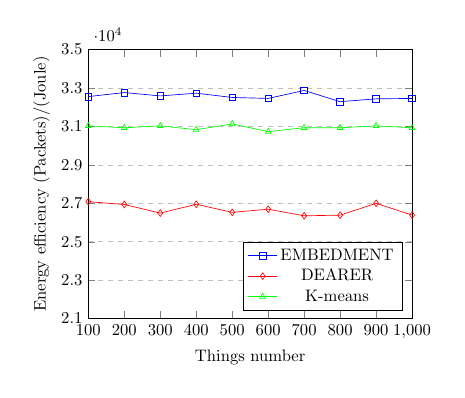
\begin{tikzpicture} [scale = 0.6]
\begin{axis}[
    %title={Energy Efficiency},
    xlabel={Things number},
    ylabel={Energy efficiency (Packets)/(Joule)},
    xmin=100, xmax=1000,
    ymin=21000, ymax=35000,
    xtick={100,200,300,400,500,600,700,800,900,1000},
    ytick={21000,23000,25000,27000,29000,31000,33000,35000},
    legend pos=south east,
    ymajorgrids=true,
    grid style=dashed,
]
  
\addplot[
    color=blue,
    mark=square,
    ]
    coordinates {
    (100,32554)(200,32764)(300,32589)(400,32731)(500,32509)(600,32458)(700,32873)(800,32289)(900,32437)(1000,32458)
    };
    \addlegendentry{EMBEDMENT}
    
\addplot[
    color=red,
    mark=diamond,
    ]
    coordinates {
    (100,27085)(200,26939)(300,26489)(400,26949)(500,26529)(600,26693)(700,26349)(800,26383)(900,26999)(1000,26388)
    };
    \addlegendentry{DEARER}
    
\addplot[
    color=green,
    mark=triangle,
    ]
    coordinates {
    (100,31031)(200,30931)(300,31031)(400,30831)(500,31131)(600,30731)(700,30931)(800,30931)(900,31031)(1000,30931)
    };
    \addlegendentry{K-means}
    
\end{axis}
\end{tikzpicture}
\end{center}
\end{figure}
\end{textblock}

\begin{textblock}{3}(8.2,0.9)
\begin{figure}[!t]
\begin{center}
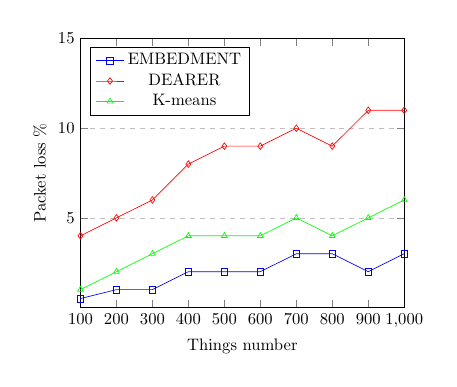
\begin{tikzpicture} [scale = 0.6]
\begin{axis}[
    %title={Packet Fail Percentage},
    xlabel={Things number},
    ylabel={Packet loss \%},
    xmin=100, xmax=1000,
    ymin=0, ymax=15,
    xtick={100,200,300,400,500,600,700,800,900,1000},
    ytick={5,10,15,20,25,30},
    legend pos=north west,
    ymajorgrids=true,
    grid style=dashed,
]
 
\addplot[
    color=blue,
    mark=square,
    ]
    coordinates {
    (100,0.5)(200,1)(300,1)(400,2)(500,2)(600,2)(700,3)(800,3)(900,2)(1000,3)
    };
    \addlegendentry{EMBEDMENT}
    
\addplot[
    color=red,
    mark=diamond,
    ]
    coordinates {
    (100,4)(200,5)(300,6)(400,8)(500,9)(600,9)(700,10)(800,9)(900,11)(1000,11)
    };
    \addlegendentry{DEARER}   
    
\addplot[
    color=green,
    mark=triangle,
    ]
    coordinates {
    (100,1)(200,2)(300,3)(400,4)(500,4)(600,4)(700,5)(800,4)(900,5)(1000,6)
    };
    \addlegendentry{K-means}
    
\end{axis}
\end{tikzpicture}
\end{center}
\end{figure}
\end{textblock}


\begin{textblock}{3}(0.7 ,8.1)
\begin{figure}
\begin{center}
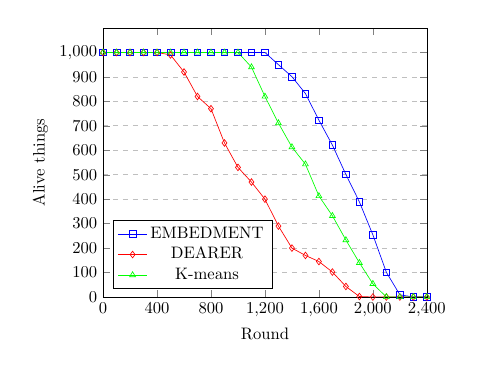
\begin{tikzpicture}[scale = 0.6]
\begin{axis}[
    %title={Packet Fail Percentage},
    xlabel={Round},
    ylabel={Alive things},
    xmin=0, xmax=2400,
    ymin=0, ymax=1100,
    xtick={0,400,800,1200,1600,2000,2400},
    ytick={0,100,200,300,400,500,600,700,800,900,1000},
    legend pos=south west,
    ymajorgrids=true,
    grid style=dashed,
]
 
 \addplot[
    color=blue,
    mark=square,
    ]
    coordinates {
    (0,1000)(100,1000)(200,1000)(300,1000)(400,1000)(500,1000)(600,1000)(700,1000)(800,1000)(900,1000)(1000,1000)(1100,1000)(1200,1000)(1300,950)(1400,901)(1500,832)(1600,723)(1700,621)(1800,501)(1900,389)(2000,254)(2100,101)(2200,9)(2300,0)(2400,0)
    };
    \addlegendentry{EMBEDMENT}
    
\addplot[
    color=red,
    mark=diamond,
    ]
    coordinates {
    (0,1000)(100,1000)(200,1000)(300,1000)(400,1000)(500,990)(600,920)(700,820)(800,770)(900,630)(1000,530)(1100,470)(1200,400)(1300,290)(1400,200)(1500,170)(1600,145)(1700,102)(1800,43)(1900,2)(2000,0)(2100,0)(2200,0)(2300,0)(2400,0)
    };
    \addlegendentry{DEARER}    
    
\addplot[
    color=green,
    mark=triangle,
    ]
    coordinates {
    (0,1000)(100,1000)(200,1000)(300,1000)(400,1000)(500,1000)(600,1000)(700,1000)(800,1000)(900,1000)(1000,1000)(1100,940)(1200,820)(1300,711)(1400,613)(1500,543)(1600,413)(1700,332)(1800,233)(1900,140)(2000,54)(2100,0)(2200,0)(2300,0)(2400,0)
    };
    \addlegendentry{K-means}
  
\end{axis}
\end{tikzpicture}
\end{center}
\end{figure}
\end{textblock}

\begin{textblock}{8}(7.5, 8.5)
\footnotesize

\begin{itemize}
\justifying
\item All factors have been improved $2.5 \times$ in Gaussian distribution compared to uniform distribution.
\item Why?
\item Average distance of things to the BS reduced app. twice.
\item Things have to send to closer BS.
\end{itemize}

\end{textblock}
\end{frame}






















\begin{frame}[t]{Third Scenario} %\vspace{10pt}

\begin{textblock}{3}(1,0.7)
\begin{figure}[!t]
\begin{center}
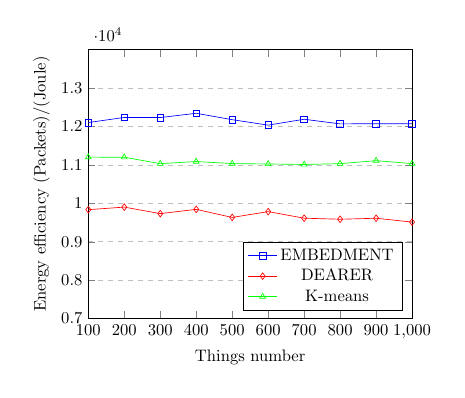
\begin{tikzpicture} [scale = 0.6]
\begin{axis}[
    %title={Energy Efficiency},
    xlabel={Things number},
    ylabel={Energy efficiency (Packets)/(Joule)},
    xmin=100, xmax=1000,
    ymin=7000, ymax=14000,
    xtick={100,200,300,400,500,600,700,800,900,1000},
    ytick={7000,8000,9000,10000,11000,12000,13000},
    legend pos=south east,
    ymajorgrids=true,
    grid style=dashed,
]
 
\addplot[
    color=blue,
    mark=square,
    ]
    coordinates {
    (100,12101)(200,12234)(300,12231)(400,12342)(500,12176)(600,12034)(700,12187)(800,12067)(900,12070)(1000,12072)
    };
    \addlegendentry{EMBEDMENT}
    
\addplot[
    color=red,
    mark=diamond,
    ]
    coordinates {
    (100,9834)(200,9901)(300,9731)(400,9842)(500,9632)(600,9784)(700,9612)(800,9585)(900,9611)(1000,9511)
    };
    \addlegendentry{DEARER}
    
\addplot[
    color=green,
    mark=triangle,
    ]
    coordinates {
    (100,11201)(200,11199)(300,11031)(400,11087)(500,11034)(600,11023)(700,11010)(800,11031)(900,11110)(1000,11033)
    };
    \addlegendentry{K-means}
    
\end{axis}
\end{tikzpicture}
\end{center}
\end{figure}
\end{textblock}

\begin{textblock}{3}(8.2,0.9)
\begin{figure}[!t]
\begin{center}
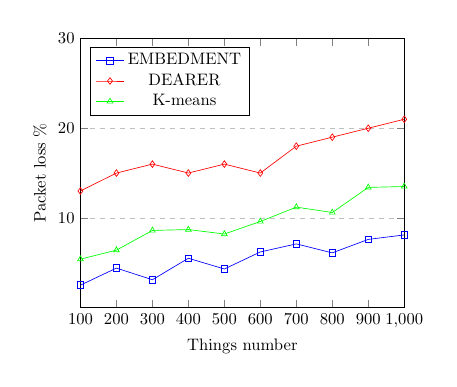
\begin{tikzpicture} [scale = 0.6]
\begin{axis}[
    %title={Packet Fail Percentage},
    xlabel={Things number},
    ylabel={Packet loss \%},
    xmin=100, xmax=1000,
    ymin=0, ymax=30,
    xtick={100,200,300,400,500,600,700,800,900,1000},
    ytick={10,20,30},
    legend pos=north west,
    ymajorgrids=true,
    grid style=dashed,
]
 
\addplot[
    color=blue,
    mark=square,
    ]
    coordinates {
    (100,2.5)(200,4.4)(300,3.1)(400,5.5)(500,4.3)(600,6.2)(700,7.1)(800,6.1)(900,7.6)(1000,8.1)
    };
    \addlegendentry{EMBEDMENT}
    
\addplot[
    color=red,
    mark=diamond,
    ]
    coordinates {
    (100,13)(200,15)(300,16)(400,15)(500,16)(600,15)(700,18)(800,19)(900,20)(1000,21)
    };
    \addlegendentry{DEARER}   
    
\addplot[
    color=green,
    mark=triangle,
    ]
    coordinates {
    (100,5.4)(200,6.4)(300,8.6)(400,8.7)(500,8.2)(600,9.6)(700,11.2)(800,10.6)(900,13.4)(1000,13.5)
    };
    \addlegendentry{K-means}
 
\end{axis}
\end{tikzpicture}
\end{center}
\end{figure}
\end{textblock}


\begin{textblock}{3}(0.7 ,8.1)
\begin{figure}
\begin{center}
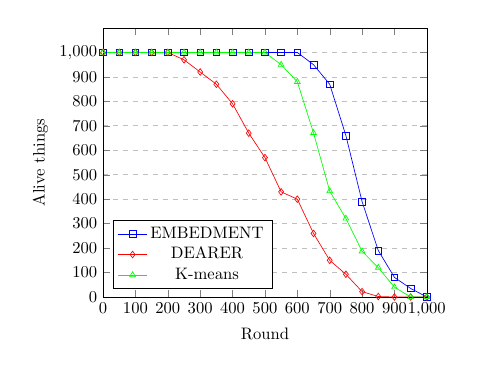
\begin{tikzpicture}[scale = 0.6]
\begin{axis}[
    %title={Packet Fail Percentage},
    xlabel={Round},
    ylabel={Alive things}, 
    xmin=0, xmax=1000,
    ymin=0, ymax=1100,
    xtick={0,100,200,300,400,500,600,700,800,900,1000},
    ytick={0,100,200,300,400,500,600,700,800,900,1000},
    legend pos=south west,
    ymajorgrids=true,
    grid style=dashed,
]
 
\addplot[
    color=blue,
    mark=square,
    ]
    coordinates {
    (0,1000)(50,1000)(100,1000)(150,1000)(200,1000)(250,1000)(300,1000)(350,1000)(400,1000)(450,1000)(500,1000)(550,1000)(600,1000)(650,950)(700,870)(750,660)(800,390)(850,190)(900,80)(950,35)(1000,0)
    };
    \addlegendentry{EMBEDMENT}
    
\addplot[
    color=red,
    mark=diamond,
    ]
    coordinates {
    (0,1000)(50,1000)(100,1000)(150,1000)(200,1000)(250,970)(300,920)(350,870)(400,790)(450,670)(500,570)(550,430)(600,400)(650,260)(700,150)(750,93)(800,22)(850,2)(900,0)(950,0)(1000,0)
    };
    \addlegendentry{DEARER}    
    
\addplot[
    color=green,
    mark=triangle,
    ]
    coordinates {
    (0,1000)(50,1000)(100,1000)(150,1000)(200,1000)(250,1000)(300,1000)(350,1000)(400,1000)(450,1000)(500,1000)(550,950)(600,880)(650,671)(700,433)(750,321)(800,187)(850,120)(900,40)(950,0)(1000,0)
    };
    \addlegendentry{K-means}
    
\end{axis}
\end{tikzpicture}
\end{center}
\end{figure}
\end{textblock}

\begin{textblock}{8}(7.5, 8.5)
\footnotesize

\begin{itemize}
\justifying
\item The results for the MG dis. are similar to uniform distribution.
\item The same average distance of things to the BS.
\item Average distance is an important factor.
\item It plays an important role in energy consumption.
\end{itemize}

\end{textblock}
\end{frame}

\begin{frame}[t]{Conclusion} %\vspace{30pt}
\begin{itemize}
\justifying
\footnotesize
\item We considered sensor data path selection problem with respect to energy consumption in the sensor layer of the IoT.
\item Current approaches fail to support:
\begin{itemize}
\item Intercluster communication, avoiding GPS
\item Residual energy, energy harvesting
\item Coverage, classic clustering
\item Distributed
\end{itemize}
\item Proposed approach support all thanks to two primary contribution:
\begin{itemize}
\item Euclidean matrix reconstruction
\item An ILP optimization problem for CH selection
\end{itemize}
\item Simulations corroborate that proposed protocol is superior considering:
\begin{itemize}
\item Energy efficiency, packet loss, lifetime
\end{itemize}
\end{itemize}
\end{frame}


\begin{frame}[t]{Questions} \vspace{30pt}
\Huge
\begin{center}
Questions?
\end{center}
\end{frame}

\begin{frame}[t]{References}
\tiny
[1] Y. Dong, J. Wang, B. Shim, and D. I. Kim, “Dearer: A distance-and-energy-aware routing with energy reservation for energy harvesting wireless sensor networks,” IEEE Journal on Selected Areas in Communications, vol. 34, no. 12, pp. 3798–3813, Dec 2016.

[2] D. Wu, J. He, H. Wang, C. Wang, and R. Wang, “A hierarchical packet forwarding mechanism for energy harvesting wireless sensor networks,” IEEE Communications Magazine, vol. 53, no. 8, pp. 92–98, August 2015.

[3] W. R. Heinzelman, A. Chandrakasan, H. Balakrishnan, Energy-efficient communication protocol for wireless microsensor networks, in: System sciences, 2000. Proceedings of the 33rd annual Hawaii international conference on, IEEE, 2000, pp. 10–pp.

[4] J. RejinaParvin and C. Vasanthanayaki, “Particle swarm optimization-based clustering by preventing residual nodes in wireless sensor networks,” IEEE Sensors Journal, vol. 15, no. 8, pp. 4264–4274, Aug 2015.

[5] A. R. Jadhav and T. Shankar, “Whale optimization based energy-efficient cluster head selection algorithm for wireless sensor networks,” CoRR, vol. abs/1711.09389, 2017. [Online]. Available: http://arxiv.org/abs/1711.09389

[6] J. Wang, K. Wang, J. Niu, W. Liu, A k-medoids based clustering algorithm for wireless sensor networks, in: 2018 International Workshop on Advanced Image Technology (IWAIT), 2018, pp. 1–4.

[7] S. Periyasamy, S. Khara, S. Thangavelu, Balanced cluster head selection based on modified k-means in a distributed wireless sensor network 2016 (2016) 1–11.

[8] S. K. Singh, P. Kumar, J. P. Singh, A survey on successors of leach protocol, IEEE Access 5 (2017) 4298–4328.

[9] Y. Miao, H. Wu, L. Zhang, The accurate location estimation of sensor node using received signal strength measurements in large-scale farmland, Journal of Sensors 2018.

[10] A. Tasissa and R. Lai, “Exact reconstruction of euclidean distance geometry problem using low-rank matrix completion,” CoRR, vol. abs/1804.04310, 2018.

\end{frame}

\begin{frame}[t]{References}
\tiny
[11] Wang, J., Wang, K., Niu, J., Liu, W. (2018). A k-medoids based clustering algorithm for wireless sensor networks. In: 2018 International Workshop on Advanced Image Technology (IWAIT), vol. 2018, pp. 1–4

[12] Periyasamy, S., Khara, S., Thangavelu, S. (2016). Balanced cluster head selection based on modified k-means in a distributed wireless sensor network. In: International Journal of Distributed Sensor Networks, vol. 2016, pp. 1–11

[13] Wang, Q., Guo, S., Hu, J., Yang, Y. (2018). Spectral partitioning and fuzzy c-means based clustering algorithm for big data wireless sensor networks. EURASIP Journal on Wireless Communications and Networking 2018(1), 54 – 65

[14] Miao, Y., Wu, H., Zhang, L. (2018). The accurate location estimation of sensor node using received signal strength measurements in large-scale farmland. Journal of Sensors 2018, 1 – 10

[15] Rasool, I., Salman, N., Kemp, A.H. (2012). Rssi-based positioning in unknown path-loss model for wsn. In: Sensor Signal Processing for Defence (SSPD 2012), pp. 1–5

[16] Yoon, Y.J., Park, W.T., Li, K.H.H., Ng, Y.Q., Song, Y. (2013). A study of piezoelectric harvesters for low-level vibrations in wireless sensor networks. International Journal of Precision Engineering and Manufacturing 14(7), 1257–1262

[17] Yang, H., Zhang, Y. (2015). Estimation of supercapacitor energy using a linear capacitance for applications in wireless sensor networks. Journal of Power Sources 275, 498 – 505

[18] Yang, H., Zhang, Y. (2011). Self-discharge analysis and characterization of superca-
pacitors for environmentally powered wireless sensor network applications. Journal of
Power Sources 196(20), 8866 – 8873

[19] Quaranta, G., Trentadue, F., Maruccio, C., Marano, G.C. (2018). Analysis of piezoelec-
tric energy harvester under modulated and filtered white gaussian noise. Mechanical
Systems and Signal Processing 104, 134 – 144

[20] A. Tasissa and R. Lai, “Exact reconstruction of euclidean distance geometry problem using low-rank matrix completion,” CoRR, vol. abs/1804.04310, 2018.

\end{frame}


\begin{frame}[t]{References}
\tiny
[21] Wang, J., Wang, K., Niu, J., Liu, W. (2018). A k-medoids based clustering algorithm for wireless sensor networks. In: 2018 International Workshop on Advanced Image Technology (IWAIT), vol. 2018, pp. 1–4

[22] Periyasamy, S., Khara, S., Thangavelu, S. (2016). Balanced cluster head selection based on modified k-means in a distributed wireless sensor network. In: International Journal of Distributed Sensor Networks, vol. 2016, pp. 1–11

[23] Wang, Q., Guo, S., Hu, J., Yang, Y. (2018). Spectral partitioning and fuzzy c-means based clustering algorithm for big data wireless sensor networks. EURASIP Journal on Wireless Communications and Networking 2018(1), 54 – 65

[24] Miao, Y., Wu, H., Zhang, L. (2018). The accurate location estimation of sensor node using received signal strength measurements in large-scale farmland. Journal of Sensors 2018, 1 – 10

\end{frame}

\end{document}